\chapter{Introduction}

% \TODO{what is a critical system, how it is different}

In critical systems such as airplanes and cars, it is important that tasks running on the hardware meet their deadlines. For example, in a car's braking system, missing a program deadline can lead to loss of control over the vehicle. Therefore, it is crucial to have a rigorous analysis that can provide an upper bound for the program's execution time on a given hardware platform. In non-critical real-time applications, the execution time bound can be estimated by measuring the execution time for many input values. This gives the maximum observed execution time, which usually underestimates the real \textit{worst-case execution time (WCET)}.

In critical real-time systems, this approach is not enough because some cases may be missed during observation, as shown in Figure \ref{fig:timing-distribution}. The real WCET can only be found by testing the program on all possible inputs, which is usually not possible due to the complexity of the state-space. Therefore, methods to estimate WCET bounds use abstractions of the program and hardware. These methods may overestimate the WCET because of simplifications, but they are more scalable.

\begin{figure}[H]
    \centering
    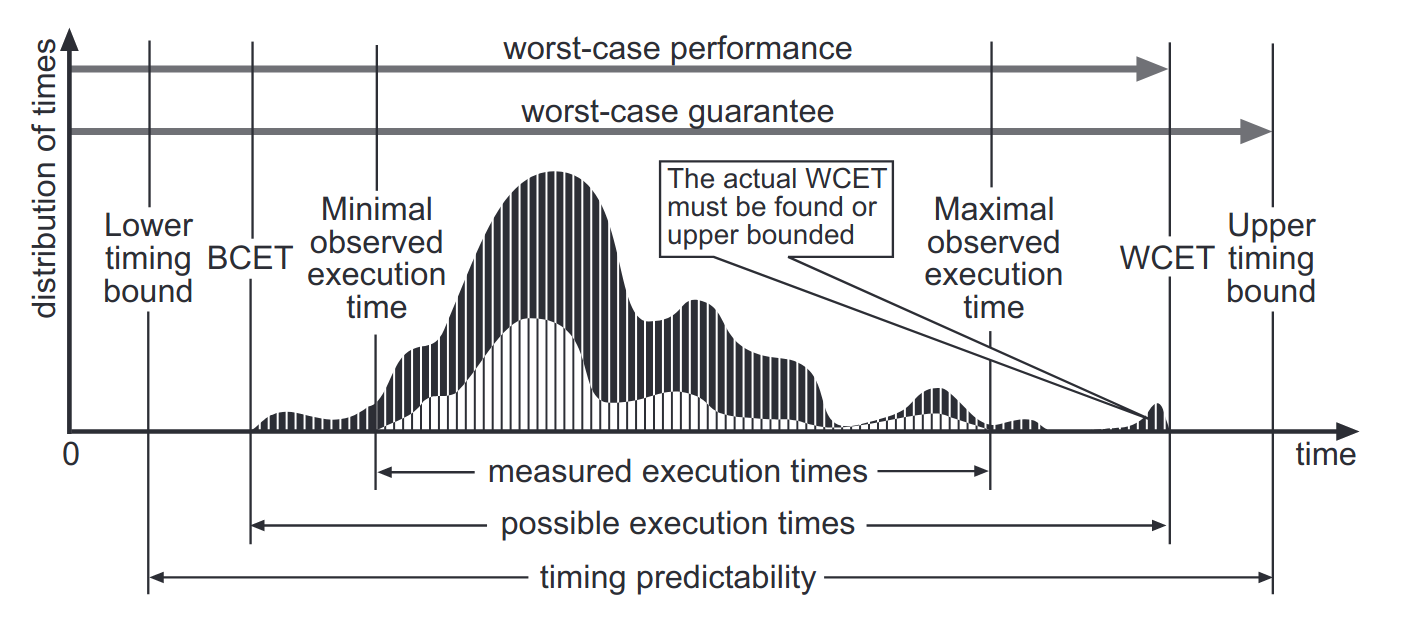
\includegraphics[width=\textwidth]{figures/timing-distribution.png}
    \caption{Timing analysis notations. The lower curve shows a subset of measured executions. The darker curve, an envelope of the former, shows the times of all executions (from \cite{ferdinand_worst_2004}).}
    \label{fig:timing-distribution}
\end{figure}

Usually, WCET analysis is divided into several phases, each focusing on a part of the hardware or software. For example, in the software part, memory analysis assigns address bounds for each instruction \cite{Harrison_Ranges_1977}, and loop bounds analysis finds the bounds for loop iterations as constants or formulas \cite{Healy_bounding_1998}. On the hardware side, there are analyzes for cache, main memory access latency, and pipeline. Together, these analyses help to find the longest path of a program, which gives the WCET bound.

\begin{figure}
    \centering
    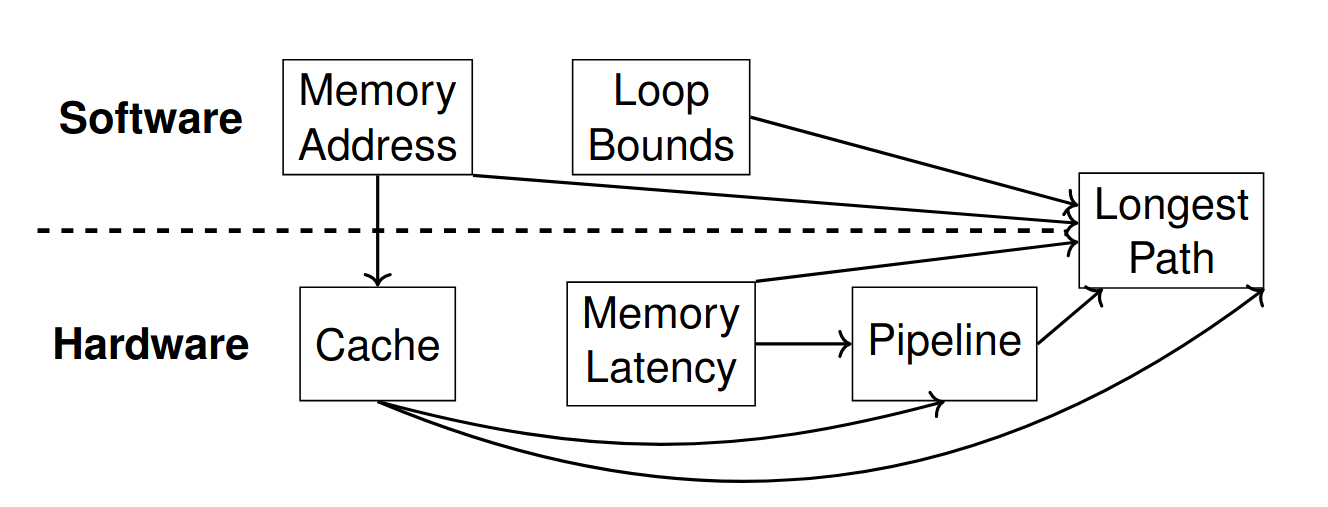
\includegraphics[width=0.7\textwidth]{figures/wcet-deps.png}
    \caption{WCET analysis phases and their dependencies. (from \cite{CAOTIC-report})}
    \label{fig:wcet-deps}
\end{figure}

Dividing WCET analysis into phases introduces the phase ordering problem: one phase may require information produced by another, leading to interdependencies. In some cases, these dependencies are circular. For instance, in Out-of-Order (OoO) processors, the instruction execution order depends on the architectural state, which also influences cache accesses. Consequently, cache analysis may depend on pipeline analysis. For timing analysis, composable systems are desirable \cite{Puschner_computing_1997}.

Nevertheless, most architectures are not composable and exhibit so-called \textit{timing anomalies (TAs)}. A TA arises when local worst-case scenarios do not necessarily lead to a global worst case. TAs are observed in pairs of execution traces with identical instruction sequences but differing initial hardware states. Variations in cache states, such as a miss in one trace and a hit in another, can result in timing differences. Example \ref{ex:simple-ta} illustrates how the initial cache state can induce a TA.

\begin{example}
Figure \ref{fig:TA1} shows an example of such an anomaly. The assembly sequence has 4 instructions ($A,B,C,D$) with data dependencies $A \rightarrow B$ and $C \rightarrow D$. Figure \ref{fig:TA1-trace} shows two traces ($\alpha, \beta$) from running the program. There is a difference in the latency of instruction $A$ ($1$ in $\alpha$ and $3$ in $\beta$). In trace $\alpha$, the variation seems better, but the total execution time is higher, which shows an anomaly.
\label{ex:simple-ta}
\end{example}

\begin{figure}[H]
    \centering
    \begin{subfigure}[t]{0.3\textwidth}
        \centering
        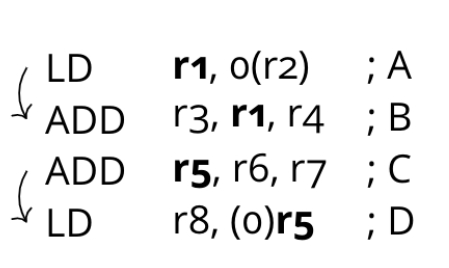
\includegraphics[width=\textwidth]{figures/first-TA-ex-input.png}
        \caption{Input assembly sequence}
        \label{fig:TA1-code}
    \end{subfigure}
    \hfill
    \begin{subfigure}[t]{0.5\textwidth}
        \centering
        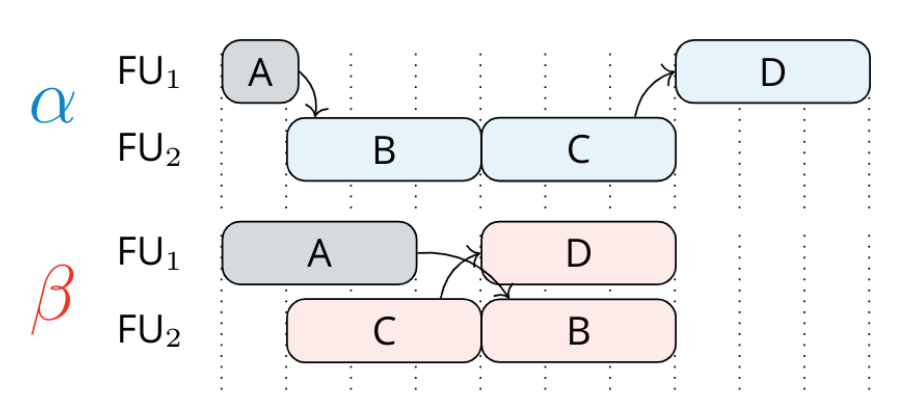
\includegraphics[width=\textwidth]{figures/first-TA-ex-trace.png}
        \caption{Scheduling on functional units}
        \label{fig:TA1-trace}
    \end{subfigure}
    \caption{TA caused by variation in latency of instruction \textit{A} (from \cite{binder_definitions_2022})}
    \label{fig:TA1}
\end{figure}

Timing anomalies pose a significant challenge for timing predictability. Understanding their nature is essential for estimating their impact on global execution time and for designing hardware that avoids TAs. Various hardware features, such as caches, memory buses, and speculative execution, can introduce TAs. In real-time systems, some of these features are often disabled to improve predictability, which can result in reduced performance. One of the most critical optimizations is branch prediction; for example, Akkas et al. \cite{Akkas2001} demonstrated that this technique can increase performance by up to $37\%$. Therefore, it is important to study the timing behavior of branch prediction to leverage its performance benefits. In this work, we focus on TAs caused by branch predictors. We begin by explaining the microarchitectural context, then review existing definitions, and finally present our framework for identifying branch-related TAs and propose a formal definition for them.
